\chapter{Diagramy ke konzoli NES}
\label{apx:ppu}

Tato příloha obsahuje dodatečné diagramy zjednodušující pochopení principu fungování konzole NES.

Diagram na obrázku~\ref{fig:ppu-renderovani} ukazuje proces vykreslování v~čipu PPU včetně operací na pozadí. V~digitální verzi jde o~vektorovou grafiku, tudíž je možné (a~doporučené) obrázek libovolně přiblížit. Pro čtenáře tištěné bakalářské práce je připravena webová verze~\cite{Nesdev:ppu-svg}.

\begin{figure}[p]
	\centering
	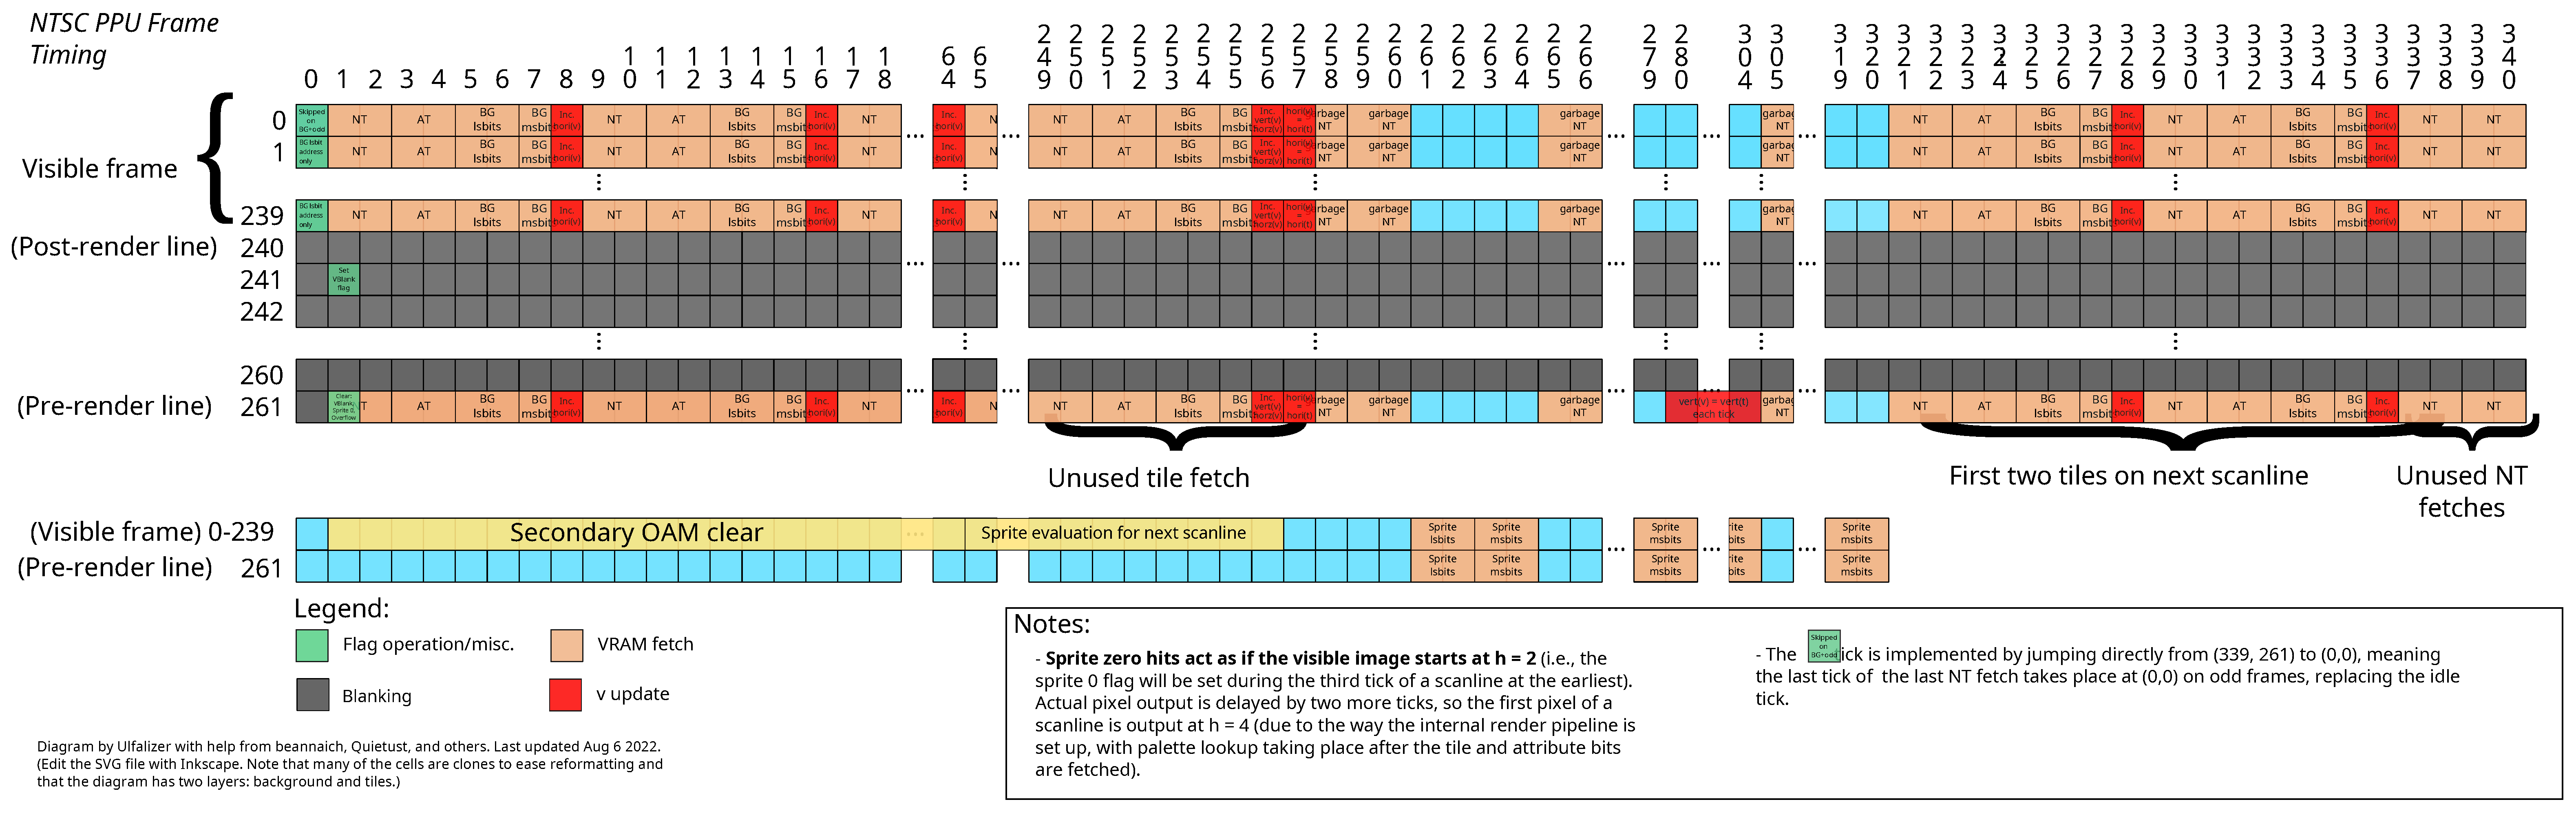
\includegraphics[width=0.98\textheight, angle=270]{images/ppudiag.pdf}
	\caption{Diagram procesu renderování u~čipu 2C02 (PPU). Vytvořila komunita Nesdev.org~\cite{Nesdev:ppu-svg}.}
	\label{fig:ppu-renderovani}
\end{figure}

\begin{figure}[p]
	\centering
	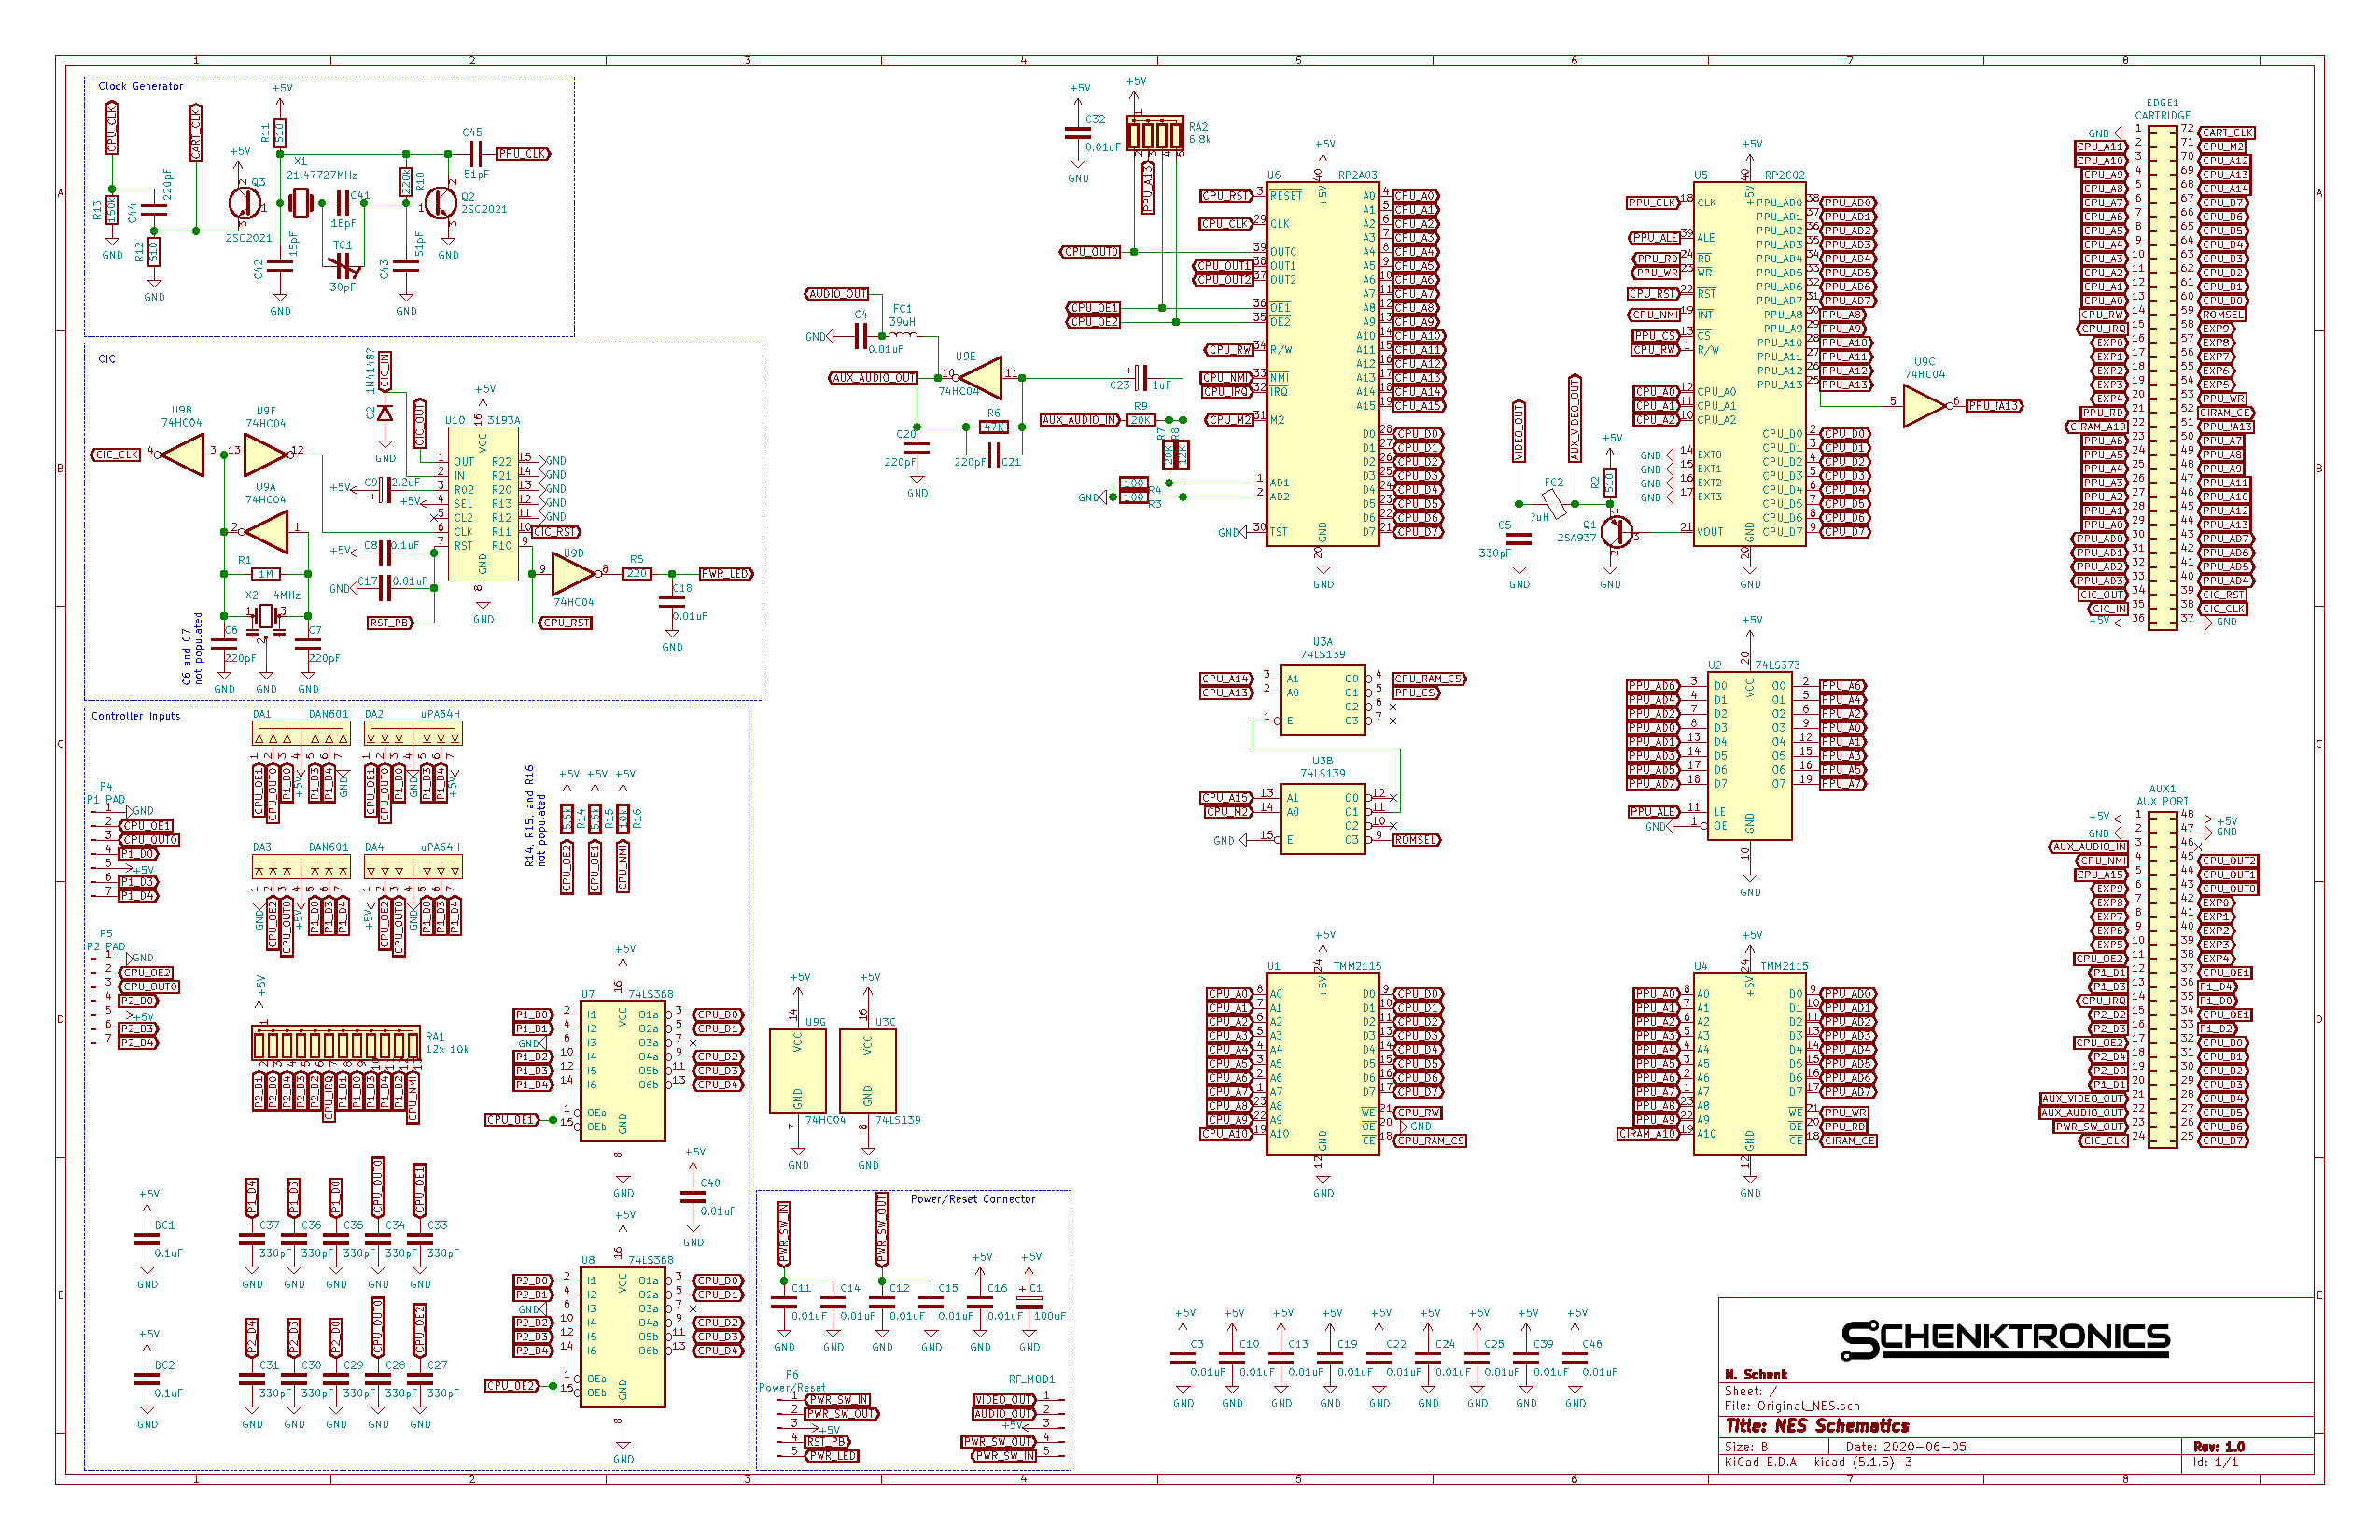
\includegraphics[width=0.92\textheight, angle=270]{images/NES-001.pdf}
	\caption{Přehledové hardwarové schéma konzole NES. Obrázek \enquote{NES-001 Console} vytvořil schenkzoola~\cite{schenkzoola2020:nes} a~zveřejnil pod licencí CC~BY~4.0.}
	\label{fig:nes001-hw}
\end{figure}

\chapter{Knihovna ImInputBinder}
\label{apx:binder}

Knihovna ImInputBinder vznikla během vývoje projektu Universal System Emulator jako rozšíření knihovny Dear~ImGui. Slouží jako centrální bod odchytávání uživatelského vstupu přes klávesnici a~herní periferie. Kromě samotného zpracování vstupu a~vyvolání akce umožňuje také změnit přiřazení kláves a~to ukládat do souboru. Návod k~použití i~samotná knihovna je k~dispozici ve veřejném repozitáři: \url{https://github.com/andreondra/ImInputBinder}, zde následuje jen meditace nad návrhovými rozhodnutími, které byly během vývoje učiněny.

První otázkou byla míra dodržování návrhových principů knihovny Dear~ImGui. Běžně jsou komponenty navrženy tak, že není nutná žádná reprezentace stavu, tedy není třeba vytvářet žádné instance tříd; stačí pouze zavolat statické metody. Ukázalo se, že aby byla komponenta konfigurovatelná, musí minimální vnitřní stav musí existovat, a to seznam akcí. Tento stav totiž vyžaduje nejen metoda pro vykreslení obrazovky nastavení přiřazení kláves, ale i~metoda pro aktualizaci stavů stisku kláves a~případné volání callbacků. I~kdyby byly principy dodrženy a~veškeré metody byly statické, musel by uživatel pomyslný vnitřní stav udržovat mimo a~dodávat jej metodám při každém volání, což je mnohem horší varianta z~hlediska výkonu, přehlednosti i~OOP principů (zapouzdřenost).

Druhou otázkou byl způsob ukládání konfigurace. Uvažovalo se nad čistě textovým formátem, pomocí něj by se snadno a~přenositelně reprezentovala čísla, avšak by mohl nastat problém u~konců řádků (znaky carriage return a line feed), což každá platforma řeší jinak. Nakonec byl zvolen vlastní (binární) formát, který většinu hodnot ukládá jako ASCII text.

\chapter{Klony NES}
\label{apx:klony-nes}
Za dobu existence konzole NES vzniklo mnoho klonů především její japonské verze Family Computer (Famicom). Tyto klony u~nás byly dosti rozšířeny na přelomu tisíciletí~\cite{Svara:polystation}. V~této příloze je pro zajímavost uvedeno několik fotografií těchto klonů. Právě díky klonům se systém NES proslavil u~nás a~dostal se takto i~do mého povědomí.

\begin{figure}[ht!]
	\centering
	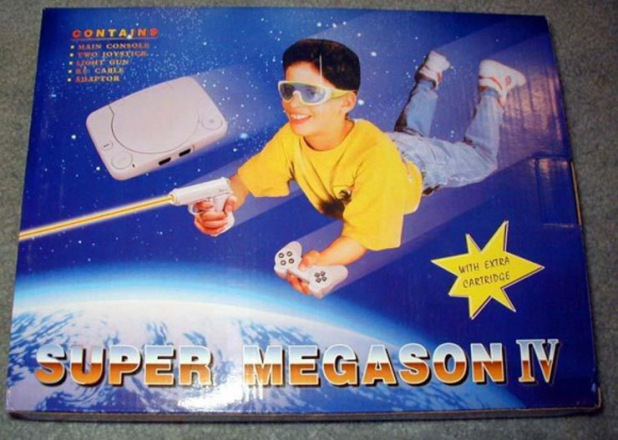
\includegraphics[width=0.5\textheight]{images/clone-megason.jpg}
	\caption{Klon \enquote{Super Megason IV} obsahující kopii periferie NES Zapper. Foto \copyright~2012 kevro, reddit.com.}
\end{figure}

\begin{figure}[ht!]
	\centering
	\includegraphics[width=0.5\textheight]{images/clone-terminator.png}
	\caption{Klon \enquote{Terminator 2} firmy \enquote{Ending-Man}. Součástí balení jsou i~pirátské kopie softwaru. Foto \copyright~2021 Tempoulker, reddit.com.}
\end{figure}

\begin{figure}[ht!]
	\centering
	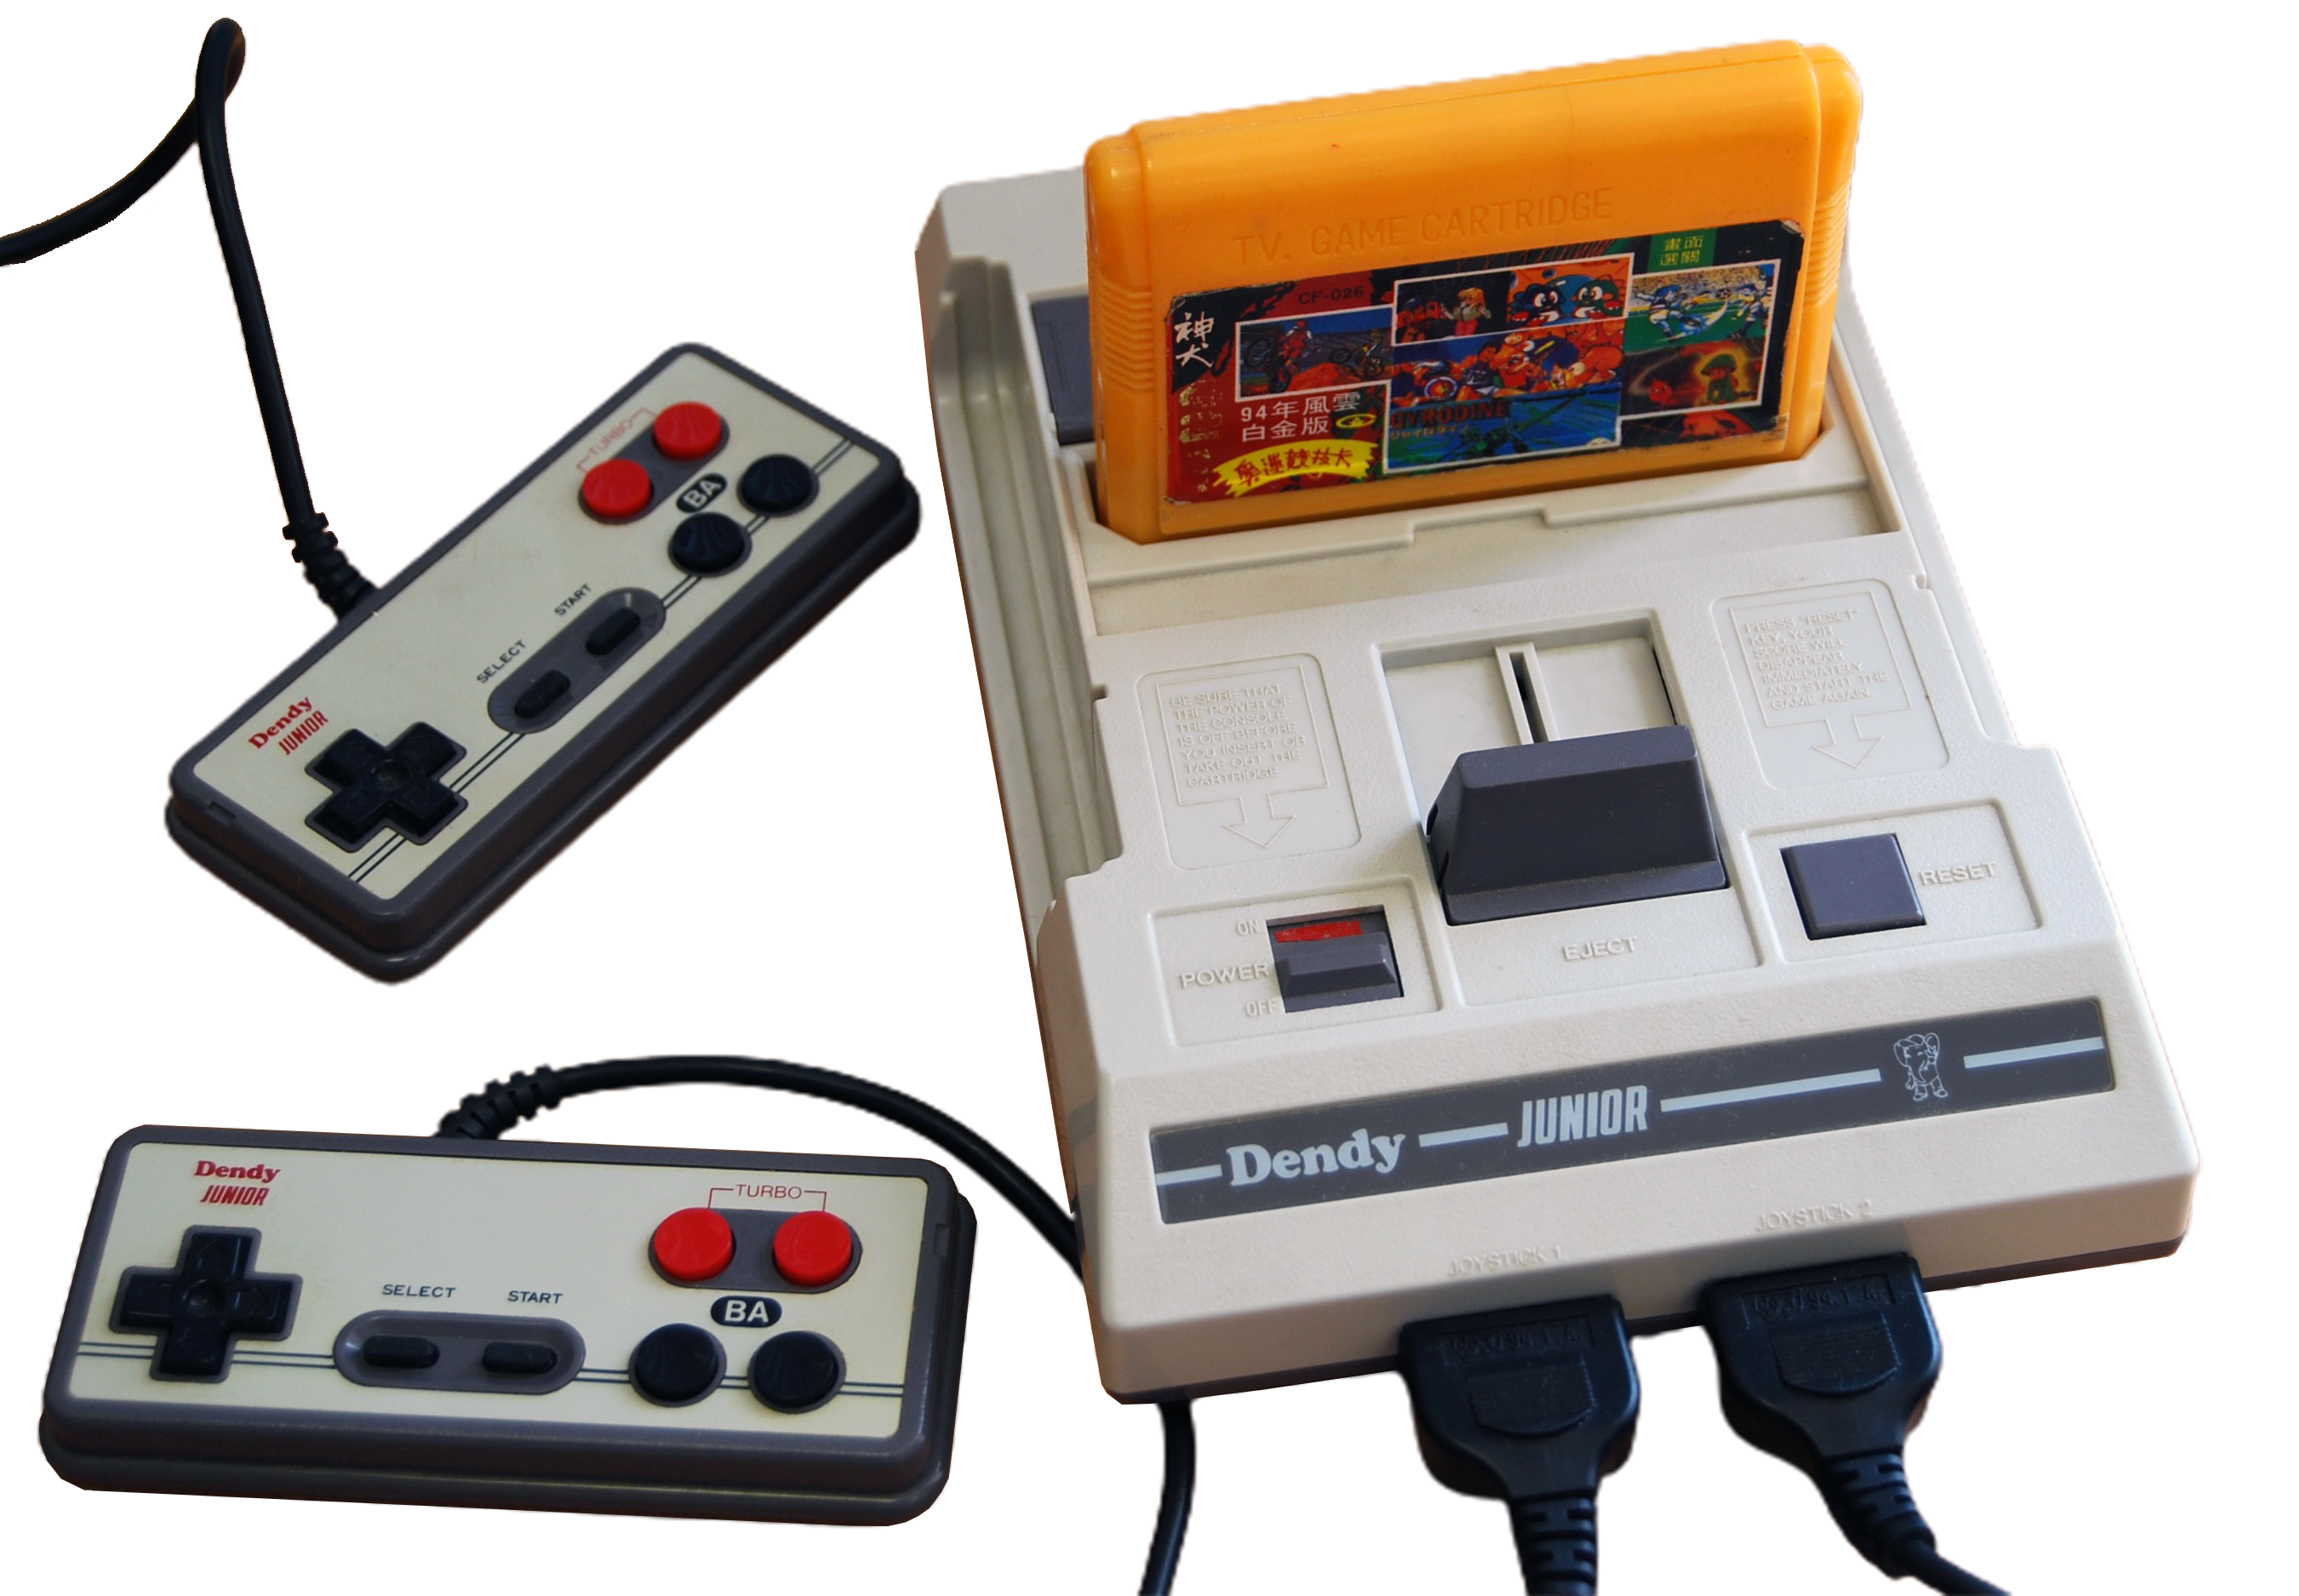
\includegraphics[width=0.5\textheight]{images/clone-dendy.png}
	\caption{Klon \enquote{Dendy Junior}, populární v~Rusku. Foto \copyright~2012 Nzeemin, wikimedia.org, CC~BY-SA~3.0, \url{https://commons.wikimedia.org/w/index.php?curid=114087394.}}
\end{figure}
